\section{Mathematical model}
First of all, it is necessary to introduce a fixed inertial reference frame $\{  \textbf{e}_1,  \textbf{e}_2,  \textbf{e}_3  \}$ and a body-fixed frame $ \{  \textbf{b}_1,  \textbf{b}_2,  \textbf{b}_3 \}$. As it was previously stated, one of the ways $\mu$MORUS UAV will exploit its shifting center of gravity (CoG) due to the moving masses in order to maneuver and stabilize itself. Therefore, a CoG vector from the origin of the body-fixed frame will be defined as follows:

\begin{equation}
	\textbf{r}_{CoG} = \frac{m_{b}\textbf{r}_{0,b} + \sum_{i=1}^n m_{i} \textbf{r}_{i}}{m_{b} + \sum_{i=1}^4 m_{i}} = \frac{\sum_{i=1}^4 m_{i}\textbf{r}_{i}}{m_t},
	\label{equ:cog}
\end{equation}

The following terms are defined as: 
\begin{itemize}
	\item $ \textbf{r}_{CoG} \in \mathbb{\text{R}}^3$ - Center of gravity with respect to the body-fixed frame
	
	\item $ \textbf{r}_{i} \in \mathbb{\text{R}}^3$ - Position of the i-th mass w.r.t. the body-fixed frame
	
	\item $ \textbf{r}_{b} \in \mathbb{\text{R}}^3$ - Position of UAV body w.r.t. the body-fixed frame. Note that because the body frame origin coincides with the rigid body CoG (without considering the moving masses) this term yields $ \textbf{r}_b = 0_{3x1}$
	
	\item $m_b \in \mathbb{R}$ - Mass of the UAV body 
	
	\item $m_i \in \mathbb{R}$ - Mass of the i-th moving mass attached to the UAV link
	
	\item $m_t \in \mathbb{R}$ - Mass of the whole UAV
\end{itemize}

When considering center of gravity in the case of UAV with the manipulator, due to the antisymmetric configuration of the links its effect on center of gravity gets mutually canceled out. The remaining formula follows:
\begin{equation}
	\textbf{r}_{CoG} = \frac{m_p\textbf{r}_l + m_p\textbf{r}_r}{m_t}
\end{equation}
where $\textbf{r}_l \in \mathbb{R}^3$ and $\textbf{r}_r \in \mathbb{R}^3$ are left and right gripper positions in the body-fixed frame. 

Moment of inertia matrix expressed in the body-fixed frame is defined as follows:
\begin{equation}
\text{J} = \text{J}_b + \sum_{i=1}^{n}\text{J}_i
\end{equation}
where $\text{J}_b$ is body and $\text{J}_i$ is moment of inertia of some mass element outside the origin of the body-fixed frame. Using the parallel axis theorem, one is able to calculate $\text{J}_i$ while knowing moment of inertia around its CoG:
\begin{equation}
\text{J}_i = \text{J}_{i,CoG} + m_i( \textbf{r}_i^T \cdot  \textbf{r}_i \text{I}_{3 \times 3} -  \textbf{r}_i \cdot  \textbf{r}_i^T)
\end{equation}
Either four moving masses or the manipulator payload will be taken in consideration when calculating each moment of inertia.

The equations of motion expressed in the inertial frame while taking in consideration that the CoG is located outside the origin of the body-fixed frame are as follows\cite{LeeModel}: 
\begin{gather}
	\dot{\textbf{x}} = \textbf{v} \label{model1}\\
	m_t\dot{\textbf{v}} + m_tg\textbf{e}_3 - m_T\text{R}  \textbf{r}_{CoG} \times \dot{\mb{\Omega}} - m_t\text{R}\hat{\mb{\Omega}}\hat{ \textbf{r}}_{CoG}\mb{\Omega} = f\text{R}\textbf{e}_3 \label{model2} \\
	\dot{\text{R}} = \text{R}\hat{\mb{\Omega}} \label{model3} \\
	\text{J} \dot{\mb{\Omega}} + \mb{\Omega} \times \text{J} \mb{\Omega} + m_t  \textbf{r}_{CoG} \times \text{R}^T \dot{\textbf{v}} = \textbf{M} \label{model4}
\end{gather}

\noindent The \textit{hat map} is an operator equivalent to the expression $\hat{x}y = \textbf{x} \times y$. It maps elements of $\mathbb{R}^3$ to the so(3) Lie algebra. \\

\noindent The following terms are defined as:

\begin{itemize}
	\item $\text{J} \in \mathbb{R}^{3 \times 3}$ - Moment of inertia matrix w.r.t. the body-fixed frame
	
	\item $\text{R} \in SO(3)$ - Rotation matrix from the body fixed frame to the inertial frame
	
	\item $\mb{\Omega} \in \mathbb{R}^3$ - Angular velocity in the body-fixed frame
	
	\item $\textbf{x} \in \mathbb{R}^3$ - Location of the body-fixed frame in the inertial frame
	
	\item $\textbf{v} \in \mathbb{R}^3$ - Velocity of the body-fixed frame in the inertial frame
	
	\item $f \in \mathbb{R}$ - Total thrust produced by the UAV
	
	\item $\textbf{M} \in \mathbb{R}^3$ - Total moments acting in the body-fixed frame
\end{itemize}

\begin{figure}[h!]
	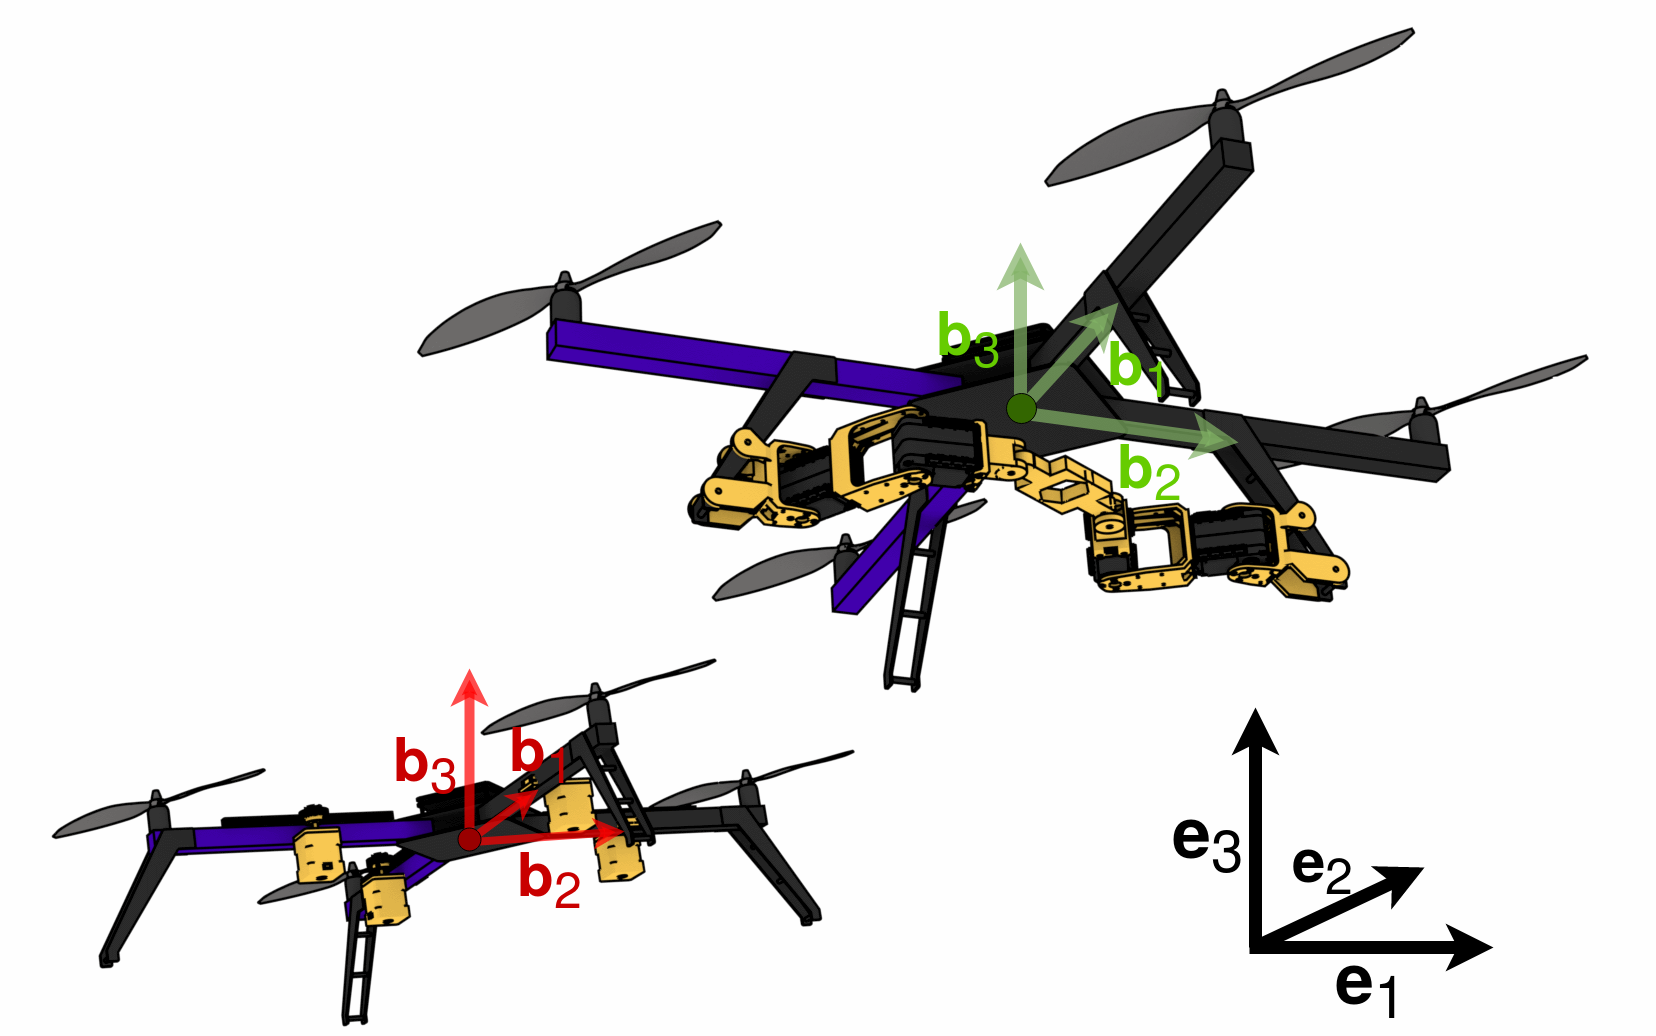
\includegraphics[width=\columnwidth]{pictures/uav.png}	
	\centering
	\label{fig:uav_model}
	\caption{UAV models with moving masses (left) and manipulators (right) along with their respective coordinate systems.}
\end{figure}

\indent Equations \ref{model1}, \ref{model2}, \ref{model3} and \ref{model4} describe the dynamical flow of a rotating and translating rigid body in terms of evolution of $(\text{R},\textbf{x},\mb{\Omega},\dot{\textbf{x}})\in \text{TSE}(3)$ on the tangent bundle of SE(3). \\
It is important to note that the changes in moment of inertia and center of gravity have been omitted in favor of simplicity in equations \ref{model2} and \ref{model4}. The complete model dynamics in the inertial frame are presented in the appendix.\\
\indent Height and yaw of the UAV is controlled by variations in rotor velocity, whereas roll and pitch by variations in center of gravity. It is assumed that first and third propeller rotate clockwise, while second and fourth rotate counter-clockwise. The relation between moments, thrust and rotor velocity is the following:
\begin{gather}
	f_i = b_f \omega_{i}^2 \label{force}\\
	\tau_i = (-1)^i b_m f_i
\end{gather}

\noindent Where the following terms are defined as:

\begin{itemize}
	\item $f_i \in \mathbb{R}$ - Thrust of the i-th motor
	
	\item $\tau_i \in \mathbb{R}$ - Moment i-th motor produces
	
	\item $b_f \in \mathbb{R}$ - Motor thrust constant
	
	\item $b_m \in \mathbb{R}$ - Motor moment constant
	
	\item $\omega_i \in \mathbb{R}$ - Rotation velocity of the i-th rotor
\end{itemize}

Total thrust can be expressed as:
\begin{equation}
	f = \sum_{1}^{4}f_i
\end{equation}
and total moment acting in the body-fixed frame as:
\begin{align}
	\begin{split}
	M = [&m_{p}gd_x  \textbf{e}_1 \cdot \textbf{b}_{3,d} , \\
	&m_{p}gd_y \textbf{e}_2 \cdot \textbf{b}_{3,d}, \\
	&b_m(-f_1 + f_2 - f_3 + f_4)]
	\end{split}
\end{align}
Using f and M as control inputs of the system one is able to obtain the desired force of each rotor and the control offset $d_x$ and $d_y$ for either moving masses or the carried payload. While the control offsets are able to be directly applied as moving mass control inputs, in the manipulator case they will be converted to infinitesimal actuator angle increments $\Delta q_1, \Delta q_2, \Delta q_3$. Such conversion will be done using the inverse Jacobian of the manipulator end effector.\\
Direct Jacobian matrix is presented as follows:
\begin{gather}
	\begin{bmatrix}
		d_x \\
		d_y
	\end{bmatrix}
	\, = \, 
	\Ja (q_1, q_2, q_3)
	\cdot 
	\begin{bmatrix}
		\Delta q_1 \\
		\Delta q_2 \\
		\Delta q_3
	\end{bmatrix} \\
	\Ja = 
	\begin{bmatrix}
		l_1\text{cos}(q_1) & l_2 \text{cos}(q_1 + q_2) & l_3 \text{cos}(q_1 + q_2 + q_3) \\
		l_1\text{sin}(q_1) & l_2 \text{sin}(q_1 + q_2) & l_3 \text{sin}(q_1 + q_2 + q_3) 
	\end{bmatrix}
\end{gather}
where $l_1$, $l_2$ and $l_3$ are the manipulator link lengths, while $q_1$, $q_2$ and $q_3$ are current actuator angles. Using Jacobian pseudinverse, incremental update rule for actuator angles can be obtained as follows:
\begin{equation}
	\begin{bmatrix}
	\Delta q_1 \\
	\Delta q_2 \\
	\Delta q_3
	\end{bmatrix} 
	\, = \, \Ja^{-1} (q_1, q_2, q_3) \cdot
	\begin{bmatrix}
	d_x \\
	d_y
	\end{bmatrix}
\end{equation}
 \\
Manipulator and moving mass actuator dynamics along with the change in desired rotor force will be regarded as instantaneous while presenting the controller synthesis and stability conditions. They will, however, be included within the Gazebo simulation environment.